\newpage
\setcounter{table}{0}
\setcounter{figure}{0}
\section{模型构建}
\subsection{建模理论依据}
根据叙事传输理论，一个高质量的众筹页面，往往在顺序上需要有严谨的递进逻辑，同时在密度上保持具有呼吸感的叙述节奏。顺序混乱会使叙事链断裂，导致用户难以构建对项目的完整认知；而节奏失控（过密或过疏）同样会使感性的叙事传输过程提前中止，受众因为视觉疲劳或感知空洞而退回理性的决策模式，说服效果随之瓦解。

本研究模型在计算层面上对上述两个维度均进行了显式建模，旨在将心理层面的“叙事质量”转化为可计算的序列特征：

\begin{enumerate}[label=(\arabic*)]
  \item 对于图文顺序，模型引入正弦位置编码，为序列中每个内容块赋予唯一的位置指纹，使 Transformer 编码器能够感知块与块之间的相对位置关系，从而捕捉不同内容出现在不同位置所蕴含的叙事语义，模拟潜在投资者在阅读项目描述时的顺序感知过程；
  \item 对于视觉密度，模型通过构建标量特征对其进行量化描述。每个内容块的类型标识（图片为1、文字为0）与物理属性（文字长度或图片面积）共同构成输入向量，Transformer 在跨块注意力计算中可以感知局部窗口内的图文分布比例与长度、大小的起伏，进而学习到与视觉密度相关的判别模式。
\end{enumerate}

通过这种理论驱动的建模方式，本研究模型不仅能识别众筹界面的表达内容，更具备了分析内容呈现逻辑的能力，从而得以实现对众筹成功性的精准预测。

\subsection{任务定义与模型概述}
\subsubsection{任务形式化定义}
本研究将众筹项目的成功预测建模为一个二分类任务。给定一个众筹项目样本，预测目标为判断该项目在筹款周期结束后能否达到预定的筹资目标。这种任务表达形式遵循了主流奖励式众筹平台（如 Kickstarter 和 Indiegogo）所采用的“全有或全无（All-or-Nothing）”策略：只有当项目在规定期限内筹得的资金总额大于或等于预设的目标金额时，项目才会被判定为成功，发起者可以获得众筹资金；否则，资金将退还给投资者，项目也将被判定为失败。

形式化表述如下：设标签为 $ y\in\{0,1\} $，其中 $ y=1 $ 表示项目成功（即最终筹款金额达到或超过筹资目标），$ y=0 $ 表示项目失败。模型的目标是学习一个映射函数，使预测值尽可能接近真实标签。具体而言，模型通过学习项目元数据、图片或文本中蕴含的多维特征，输出标量预测值 Logit $ z\in\mathbb{R} $，并最终通过 Sigmoid 激活函数将该值映射到$ (0,1) $区间，得到项目成功的预测概率：
\begin{equation}
\hat{p}=\sigma(z)=\frac{1}{1+\exp(-z)}.
\end{equation}
在模型训练阶段，预测概率与真实标签之间的差异通过二分类交叉熵（Binary Cross Entropy, BCE）损失函数进行度量。训练目标为最小化该损失函数，从而驱动模型捕捉众筹页面和元数据中与项目筹资结果相关的深层判别模式。

\subsubsection{模型架构概述}
本研究构建了一个基于统一序列建模范式的多模态深度学习模型 MSTC（Multimodal Sequential Transformer for Crowdfunding），主要分为三部分：

\begin{enumerate}[label=(\arabic*)]
  \item 多模态序列构建：模型首先将众筹页面的非结构化内容转化为有序序列。利用预训练 CLIP 模型作为统一后端，提取图文对齐的语义特征。为捕捉页面布局的物理线索，模型除语义向量外还加入了视觉密度（文本长度、图片面积）与模态类型特征，并按网页 DOM 树的真实顺序构建多模态 Token 序列，从而真实还原投资者的线性阅读过程。
  \item 叙事逻辑建模：采用 Transformer Encoder 作为核心序列编码器。通过正弦位置编码赋予模型感知图文顺序的能力，并利用自注意力机制跨模态融合图文信息，系统性地捕捉页面呈现中的叙事逻辑。
  \item 异构特征融合与预测：模型聚合序列特征后得到反映项目整体印象的内容表示向量，该向量随后与项目的静态元数据分支进行特征融合，最终由分类头输出项目成功性预测结果。
\end{enumerate}


\begin{figure}[H]
  \centering
  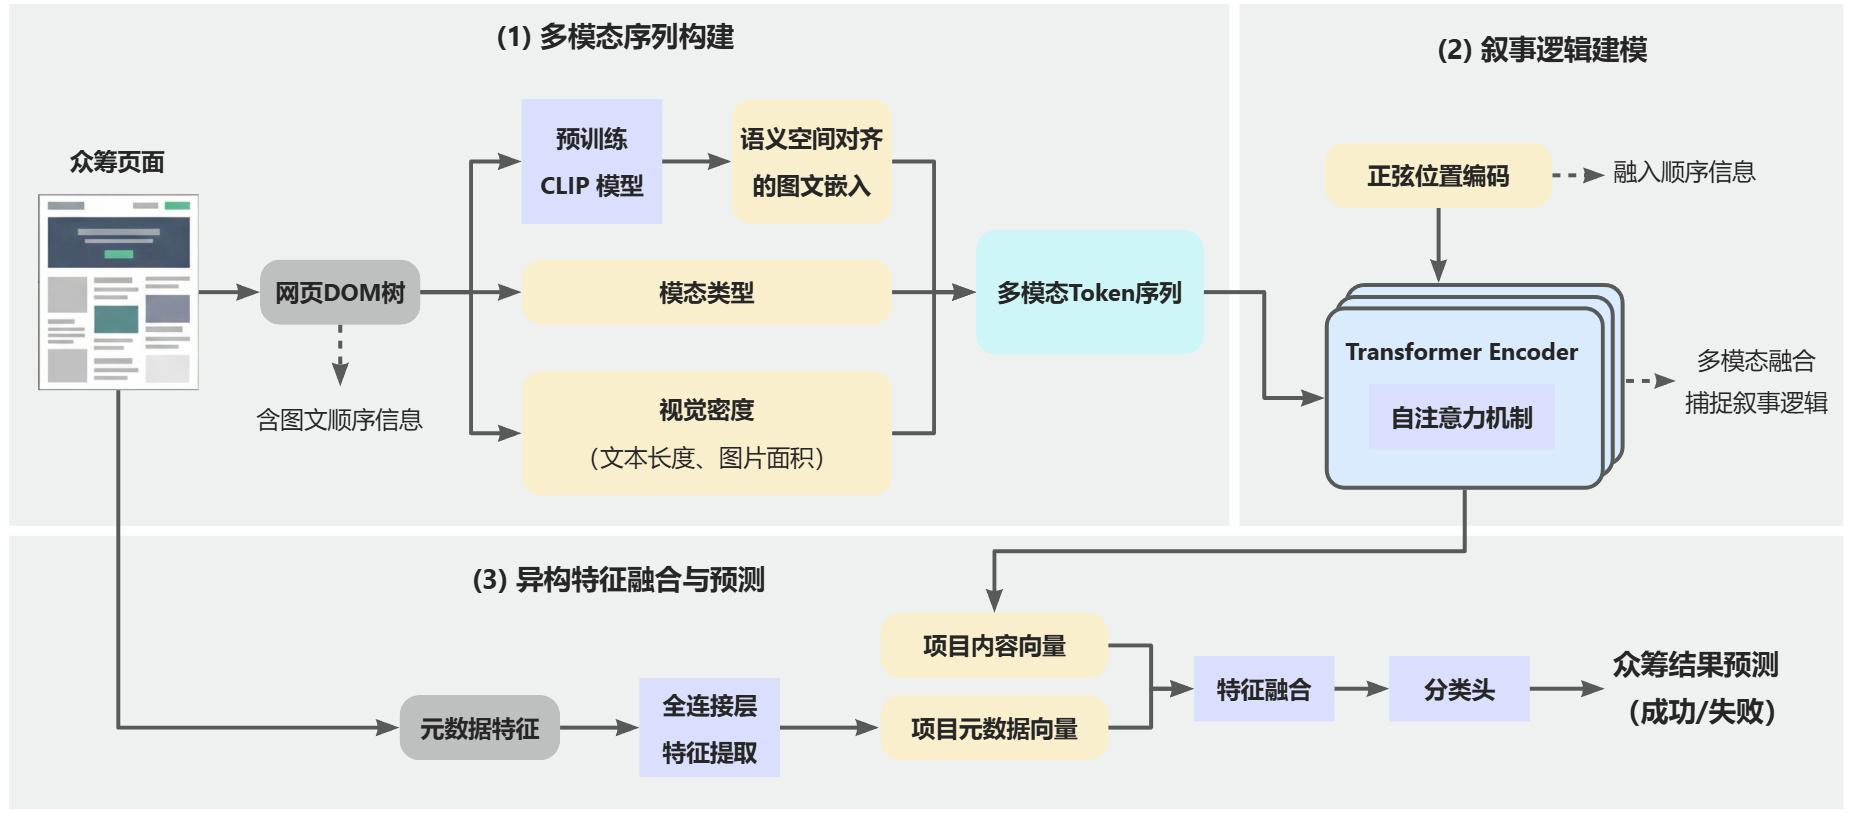
\includegraphics[width=0.95\textwidth]{figures/MSTC_overview.jpg}
  \caption{MSTC 模型架构概览}
  \label{fig:mstc_overview}
\end{figure}

\subsection{多模态数据表征与图文序列构建}
为了模拟投资者在众筹页面上的“叙事传输”体验，模型需要将非结构化的网页内容转化为具备顺序特征和物理属性的结构化输入。本节详细说明如何将文本、图像及布局属性编码为统一的多模态序列。

\subsubsection{多模态语义表征}
本研究的多模态输入由文本与图像的特征向量共同构成。为解决多模态融合中常见的语义空间不一致问题，消除建模时模态间的语义鸿沟，本研究通过统一嵌入后端、各模态差异化向量生成及离线固定表征等环节，构建了标准化的特征提取流程。

实现多模态语义表征的核心在于引入预训练的 CLIP 模型作为图像与文本的向量化后端。通过在 4 亿规模的图像-文本对数据集上进行对比学习，CLIP 模型将视觉编码器和文本编码器映射至同一个对齐的特征空间中，使得生成的图文向量在语义维度上天然对齐，下游序列模型可以忽略底层模态差异，专注于捕捉跨模态叙事逻辑。在具体模型版本选择上，本研究采用 OpenAI 开源的 ViT-B/32 版本。其视觉编码器采用 Vision Transformer 架构，将输入图像划分为$ 32 \times 32 $像素的补丁（Patches）进行全局特征提取；文本编码器采用 Transformer 架构，利用自注意力机制对文本 Token 进行语义建模。向量化后图像向量与文本向量维度一致，均为 $ D_{\text{img}}=D_{\text{txt}}=512 $。

在向量生成机制的设计上，为了确保特征提取的质量，本研究针对不同模态的特性设计了不同的向量化流程。对于项目封面图及正文图像，首先将其转换为 RGB 格式并进行标准化的尺寸缩放，随后提取 512 维的全局视觉特征向量，并对其进行$ L_2 $归一化处理，以消除非语义因素对特征分布的影响。对于文本，由于文本编码器存在 77 个 Token 的硬性长度限制，而众筹项目中有大量长文本内容，本研究设计了基于滑动窗口的表征机制。首先，将长文本按照最大窗口长度切分为多个重叠的内容片段，每次滑动的步长设定为 32 个 Token，确保片段间的上下文连续性；随后对同一文本块生成的多个片段特征向量执行均值池化，并对结果再次进行$ L_2 $归一化，从而获得能够覆盖整段文本信息的表征向量。

后续训练使用的所有图文向量均在训练前离线生成并保持固定，训练阶段不再微调模态编码器，仅加载对应向量参与建模。这一设定旨在排除嵌入模型底层编码能力的差异，使实验差异集中在模型结构而非模态编码器能力上，确保实验性能的提升完全源于模型对众筹内容呈现逻辑的捕捉能力，保证对比实验的公平性。

最后，本研究选取图文信息时遵循以下原则：对于每个项目，文本侧信息包含标题、简介以及正文内容块中的多段文本；图像侧信息包含封面图以及正文中的多张图片。

\subsubsection{视觉密度特征提取}
为了量化加工流畅性理论中的“视觉密度”特征，本研究为序列中的每个位置定义了辅助信息向量：对每个位置 $ i\in\{1,\ldots,L\} $，定义类型标识 $ t_i\in\{0,1\} $（文本为 0，图片为 1）、标量属性 $ a_i\in\mathbb{R} $。每个内容块的标量属性 $ a $ 为其结构信息，用于提供与视觉密度相关的粗粒度物理线索。针对不同模态，标量属性的计算方式如下：

\begin{enumerate}[label=(\arabic*)]
  \item 对于文本块，令 $ \ell $ 为文本长度，通过对数变换平滑长尾分布：
  \begin{equation}
  a=\log(\max(1,\ell));
  \end{equation}
  \item 对于图片块，令 $ w,h $ 为图片的分辨率宽高，则其面积为 $ \text{area}=w\cdot h $，同理进行对数处理：
  \begin{equation}
  a=\log(\max(1,\text{area})).
  \end{equation}
\end{enumerate}


通过将语义向量与上述结构属性相融合，模型能够同时感知“叙事内容”与“呈现节奏”，从而更精准地预测投资者的决策反馈。

\subsubsection{叙事序列构建}
基于线性叙事理论，本研究放弃了传统的晚期融合范式，转而将页面内容抽象为符合人类浏览顺序的统一序列。序列由固定前缀与正文内容块组成，前缀包含标题、简介与封面图；随后按页面呈现顺序，即 HTML DOM 树中真实的物理展示顺序拼接正文中的图文块。

为模拟用户在有限注意力下的前部窗口浏览行为，并平衡计算效率，本研究设定块长度上限为 40（ 即 $ L_{\max}=40 $），并固定取页面前部窗口。前缀长度固定为 3，设正文长度为 $ L_{\text{body}} $，则截断前序列长度为 $ 3+L_{\text{body}} $，统一后的序列实际长度为：
\begin{equation}
L=\min(3+L_{\text{body}},L_{\max})
\end{equation}
\subsection{统一序列预测模型设计}
本研究构建了一个基于统一序列建模范式的多模态深度学习模型 MSTC。模型的核心思想是将项目内容表示为统一的图文 Token 序列，通过 Transformer 显式建模 Token 间的叙事交互，并融合元数据进行预测。

\subsubsection{Token 编码器}
为了将异构的语义向量、类型信息与物理属性整合为统一的隐藏层表示，本研究在模型的 Token 编码器模块构建了一套层次化的特征融合流程。

模态投影作为流程的起点，旨在消除不同原始模态间的量纲差异。设第 $ i $ 个位置的图像与文本嵌入向量分别为 $ e_i^{\text{img}}\in\mathbb{R}^{512} $ 与 $ e_i^{\text{txt}}\in\mathbb{R}^{512} $。模型首先对两种模态分别做线性投影并经 ReLU 激活：
\begin{equation}
u_i^{\text{img}}=\text{ReLU}(W_{\text{img}}e_i^{\text{img}}+b_{\text{img}}),\quad
u_i^{\text{txt}}=\text{ReLU}(W_{\text{txt}}e_i^{\text{txt}}+b_{\text{txt}}),
\end{equation}
其中权重矩阵 $ W_{\text{img}},W_{\text{txt}}\in\mathbb{R}^{256\times 512} $。

在获得投影向量后，模型依据输入序列中的类型标识动态选择有效的模态投影，确保对应位置仅保留所属模态的特征表达：
\begin{equation}
u_i=\mathbb{I}[t_i=1]\cdot u_i^{\text{img}}+\mathbb{I}[t_i=0]\cdot u_i^{\text{txt}}.
\end{equation}
模型通过类型与属性注入进一步丰富 Token 的上下文含义。为了显式区分图像块与文本块，本研究引入了可学习的类型嵌入表 $ E_{\text{type}}\in\mathbb{R}^{2\times 256} $，显式编码该位置的类型，通过查表操作获取类型编码：
\begin{equation}
v_i=E_{\text{type}}(t_i).
\end{equation}
属性标量通过线性层投影到隐藏空间，转化为能够与语义特征对齐的维度：
\begin{equation}
w_i=W_{\text{attr}}a_i+b_{\text{attr}},\quad W_{\text{attr}}\in\mathbb{R}^{256\times 1}.
\end{equation}
整个编码过程汇聚于特征融合层，最终 Token 表示定义为三者相加后的正则化输出：
\begin{equation}
x_i=\text{Dropout}\big(\text{LayerNorm}(u_i+v_i+w_i)\big),
\end{equation}
其中 Token 级 Dropout 取 0.33。

综上所述，图文序列通过 Token 编码器后得到序列张量 $ X\in\mathbb{R}^{B\times L_{\max}\times 256} $，为后续建模奠定了数据基础。

\subsubsection{正弦位置编码}
在图文 Token 序列进入 Transformer 序列编码器前，必须赋予模型感知呈现顺序的能力，以模拟投资者沿纵向页面浏览时的线性感知过程。为显式刻画图文块的先后排列关系，本研究在序列中注入固定的正弦位置编码（Position Encoding）。对位置 $ p\in\{0,\ldots,L_{\max}-1\} $ 与维度索引 $ k $，编码定义如下：
\begin{equation}
\text{PE}(p,2k)=\sin\left(\frac{p}{10000^{2k/d}}\right),\quad
\text{PE}(p,2k+1)=\cos\left(\frac{p}{10000^{2k/d}}\right),
\end{equation}
在有效位置上进行元素级相加，得到增强顺序感知的输入向量：
\begin{equation}
x'_i=x_i+m_i\cdot \text{PE}(p=i-1).
\end{equation}
该设计确保了模型对图文顺序的识别能力：若不加位置编码，则 Transformer 架构退化为对无序 Token 集合的处理；而加入位置编码后，模型具备表达相对位置与顺序模式的能力，从而可用于检验顺序信息的边际贡献。

\subsubsection{Transformer 序列编码器}
位置编码后的图文 Token 序列进入 Transformer 编码器。该模块通过多头自注意力机制模拟读者在阅读过程中不断回溯上下文、印证图文逻辑的认知行为。

编码器由两层编码层堆叠构成，每层隐藏维度位 $ d=256 $，多头数 $ H=4 $（每头维度 $ d_k=64 $），前馈网络中间维度 $ d_{\text{ff}}=512 $，Dropout 率为 0.1，采用 pre-LN 结构以提升训练稳定性。

设第 $ \ell $ 层输入为 $ Z^{(\ell-1)}\in\mathbb{R}^{B\times L_{\max}\times 256} $， 则单层编码过程定义为：
\begin{equation}
\tilde{Z}^{(\ell)}=Z^{(\ell-1)}+\text{MHA}(\text{LN}(Z^{(\ell-1)})),
\end{equation}
\begin{equation}
Z^{(\ell)}=\tilde{Z}^{(\ell)}+\text{FFN}(\text{LN}(\tilde{Z}^{(\ell)})),
\end{equation}
其中多头注意力的核心计算如下：
\begin{equation}
\begin{aligned}
\text{MHA}(x)&=\text{Concat}(\text{head}_1,\ldots,\text{head}_H)W^O,\\
\text{head}_h&=\text{softmax}\left(\frac{Q_hK_h^\top}{\sqrt{d_k}}\right)V_h.
\end{aligned}
\end{equation}
前馈网络定义为：
\begin{equation}
\text{FFN}(x) = W_2\text{ReLU}(W_1x + b_1) + b_2
\end{equation}
经过两层编码，模型输出蕴含了深度跨模态交互信息的序列表示 $ Z\in\mathbb{R}^{B\times L_{\max}\times 256} $。

\subsubsection{融合分类}
通过 Transformer 编码器捕获 Token 间的叙事交互后，模型需要将局部的、动态的序列信息聚合为全局的项目表征，并结合结构化元数据给出最终的预测结果。

为了从图文交替的叙事流中提取出反映项目整体质量的特征向量，本研究对 Transformer 输出的序列表示进行屏蔽均值池化（Masked Mean Pooling），得到项目级内容表示$ h\in\mathbb{R}^{256} $：
\begin{equation}
h=\frac{\sum_{i=1}^{L_{\max}} m_i z_i}{\sum_{i=1}^{L_{\max}} m_i},
\end{equation}
其中 $ z_i $ 表示 $ Z $ 在位置 $ i $ 的向量。该设计模拟了投资者在阅读完整个页面后形成的综合印象。

除了页面内容呈现的叙事价值外，项目的先天背景（如目标金额、持续时间）也是影响决策的关键因素。本研究将 155 维的结构化元数据特征$ x_{\text{meta}}\in\mathbb{R}^{155} $， 输入一层多层感知机（MLP）进行非线性映射，得到元数据表示：
\begin{equation}
h_{\text{meta}}=\text{Dropout}\big(\text{ReLU}(W_{\text{meta}}x_{\text{meta}}+b_{\text{meta}})\big),
\end{equation}
其中隐藏层维度为 128，Dropout 为 0.2，故 $ h_{\text{meta}}\in\mathbb{R}^{128} $。

将代表图文序列整体叙事的向量与代表项目属性的元数据向量进行拼接，形成最终的融合表征向量：
\begin{equation}
f=[h;h_{\text{meta}}]\in\mathbb{R}^{384}.
\end{equation}
分类头负责将融合后的多维特征映射为预测空间。为了提升训练稳定性并防止过拟合，本研究采用了两层全连接结构并引入层归一化（LayerNorm）：
\begin{equation}
\tilde{f}=\text{LN}(f),\quad
g=\text{Dropout}\big(\text{ReLU}(W_f\tilde{f}+b_f)\big),\quad
z=w^\top g+b,
\end{equation}
其中 $ W_f $ 将输入映射到 512 维隐藏层， Dropout 率为 0.5，最终输出标量 Logit$ z $, 代表该众筹项目成功预测的原始得分。

\subsubsection{模型总体结构}
本节构建了一个整合多模态内容序列与项目元数据的众筹成功预测模型 MSTC，它通过两条并行的特征提取路径实现了对众筹项目的深度表征。模型的完整逻辑架构及内部参数如图 3-2 所示。


\begin{figure}[H]
  \centering
  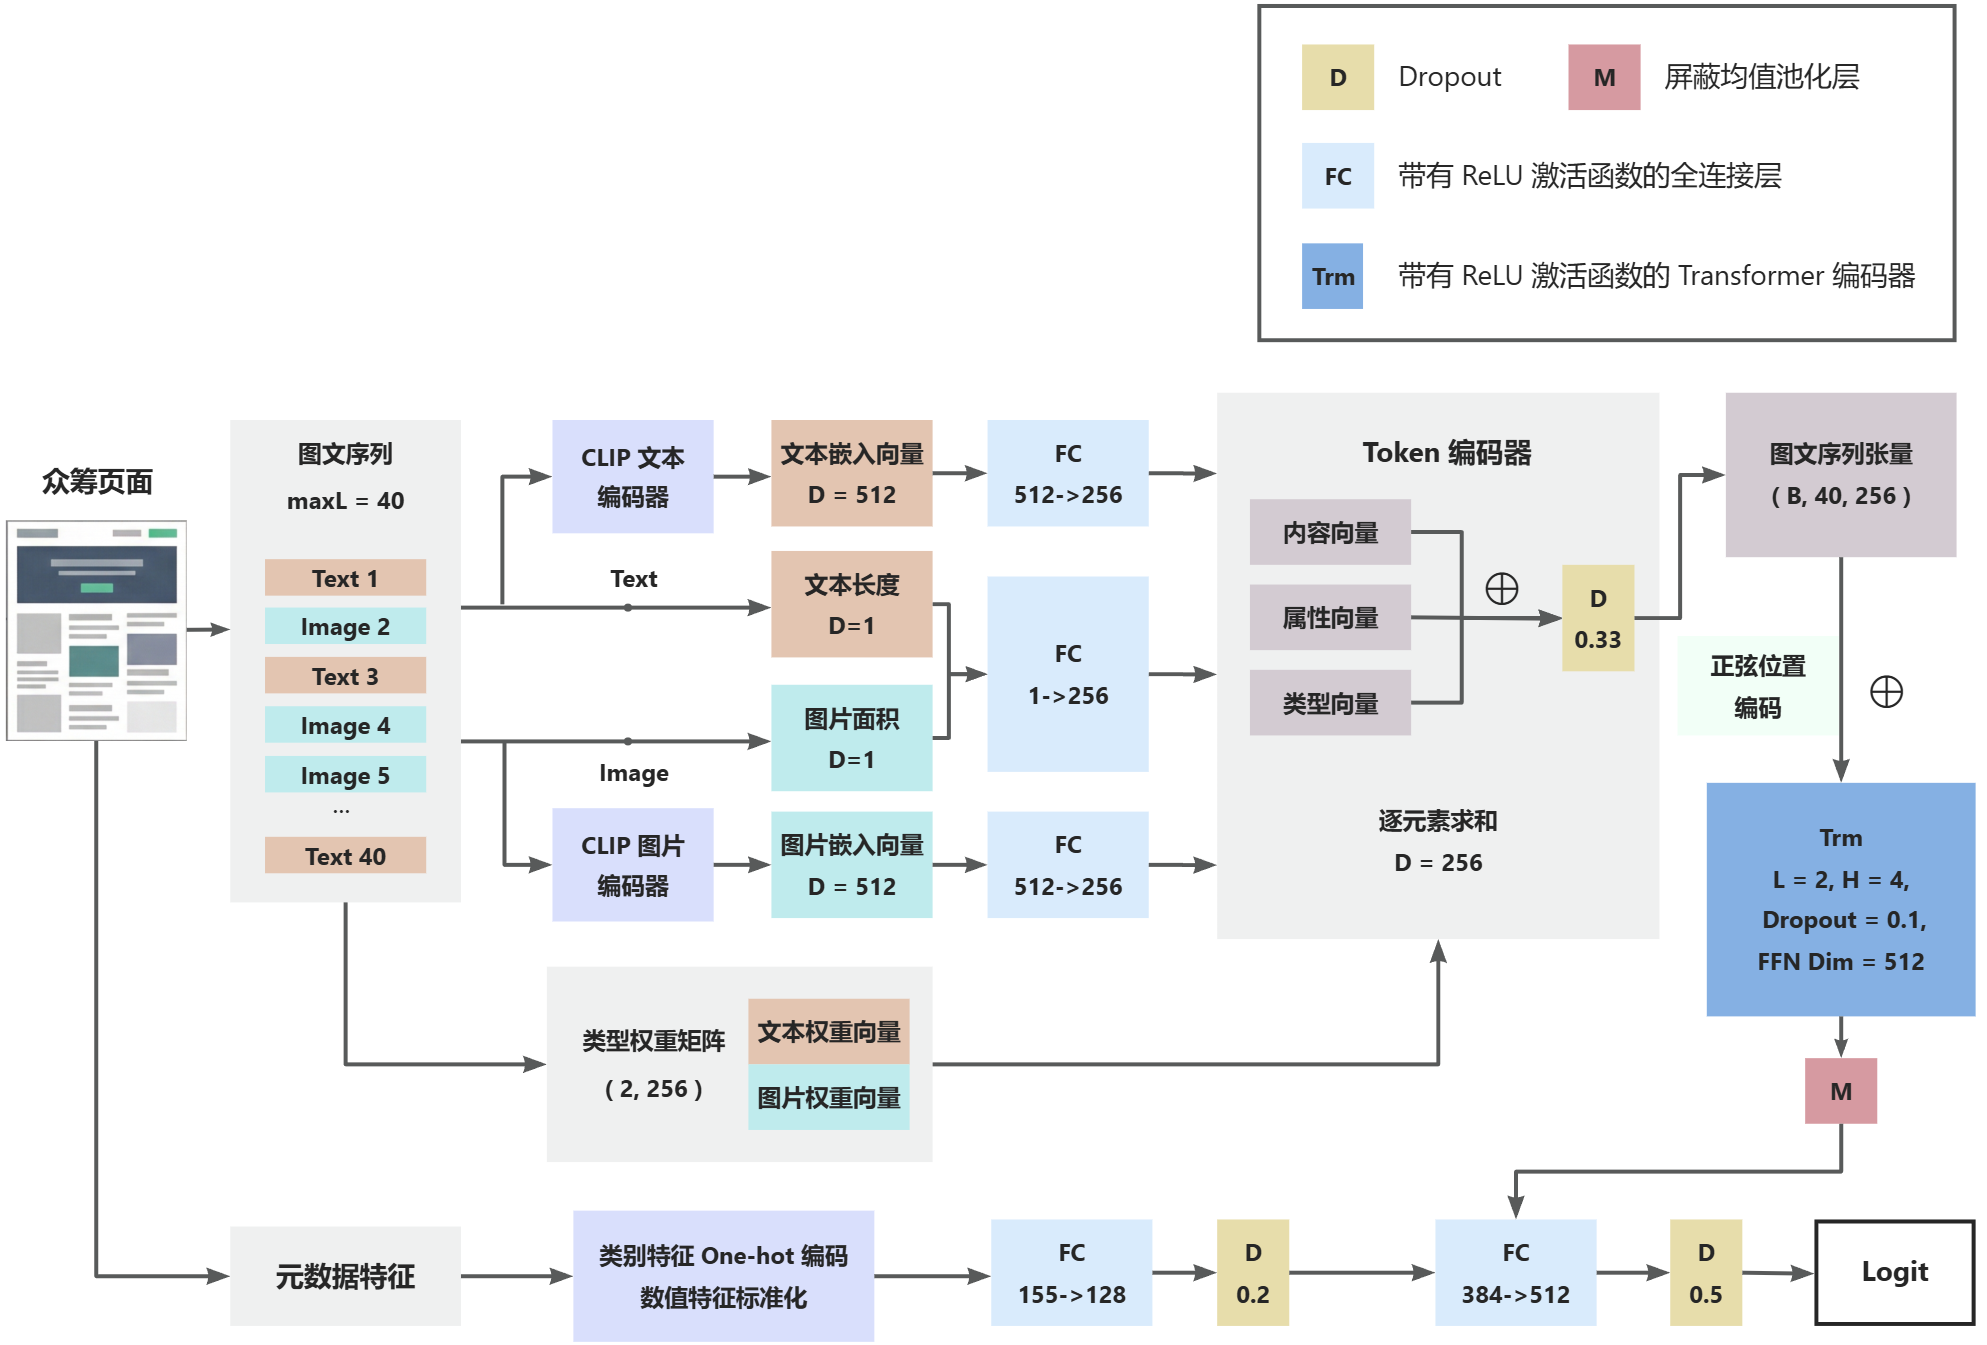
\includegraphics[width=0.95\textwidth]{figures/MSTC_param.jpg}
  \caption{MSTC 模型结构参数图}
  \label{fig:mstc_param}
\end{figure}

\subsection{训练目标与优化策略}
\subsubsection{概率输出与损失函数}
本研究将众筹成功性预测建模为二分类任务。模型末层输出原始分数 Logit$ z $并通过 Sigmoid 函数映射为预测概率$ \hat{p}=\sigma(z) $。采用二分类交叉熵作为目标损失函数，以衡量预测分布与真实分布之间的差异：
\begin{equation}
\mathcal{L}=-\frac{1}{N}\sum_{i=1}^{N}\left(\tilde{y}_i\log \hat{p}_i+(1-\tilde{y}_i)\log(1-\hat{p}_i)\right),
\end{equation}
其中 $ \tilde{y} $ 是经过标签平滑（Label Smoothing）处理后的软标签。传统的硬标签（0或1）容易导致模型在训练时过于自信，进而引发过拟合，降低验证集和测试集上的预测准确度。为缓解过拟合并提升模型表现，本研究采用平滑系数 $ \epsilon=0.05 $，对原始标签 $ y\in\{0,1\} $进行如下变换：
\begin{equation}
\tilde{y}=(1-\epsilon)y+\frac{\epsilon}{2}.
\end{equation}
通过该处理后，正类标签从 1 变为 0.975，负类标签从 0 变为 0.025，强制模型学习更具有泛化性的特征。该处理在所有对照实验中保持一致。

\subsubsection{训练配置与稳定性策略}
本研究采用了一系列策略以确保模型训练的收敛速度与推理阶段的稳定性：

\begin{enumerate}[label=(\arabic*)]
  \item 优化器选择：使用 AdamW 优化器作为模型训练的优化方案。在标准的 Adam 优化器中，$ L_2 $正则化项通常被直接合并至损失函数，正则与梯度更新耦合在一起。这种耦合会导致正则化项的实际强度随梯度变化产生波动，从而使正则化项失去预期的约束作用。

  针对这一局限性，AdamW 算法显式地将权重衰减与梯度更新解耦，使其能够以恒定的速率作用于参数更新，能够更有效地防止模型参数过大，提升正则化效果。AdamW 的核心更新流程遵循以下公式：
  \begin{equation}
  \begin{aligned}
  g_t &= \nabla_{\theta} L_t(\theta_{t-1}) ,
  \\
  m_t &= \beta_1 m_{t-1} + (1 - \beta_1) g_t, \\
  v_t &= \beta_2 v_{t-1} + (1 - \beta_2) g_t^2, \\
  \theta_t &= \theta_{t-1} - \eta_t \left( \frac{\hat{m}_t}{\sqrt{\hat{v}_t} + \epsilon} + \lambda \theta_{t-1} \right).
  \end{aligned}
  \end{equation}
  上式中，$ \eta_t $代表学习率，$ \lambda $代表预设的权重衰减系数。

  在这一更新逻辑下，权重衰减项 $ \lambda \theta_{t-1} $ 直接作用于参数更新步骤，而不参与动量与二阶矩的自适应缩放计算。这种独立的权重衰减机制确保了无论梯度如何演变，模型始终能受到恒定的参数约束，从而能够更有效地抑制模型过拟合。

  \item 学习率调度策略：为平衡训练初期的稳定性和后期的收敛精度，学习率调度采用线性预热（Warmup）配合余弦退火（Cosine Annealing）策略。设总训练步数为 $ T $，本研究将线性预热阶段比例设置为 0.1（即 Warmup 步数 $ T_w=0.1T $）。学习率随步数的变化定义如下：
  \begin{equation}
  \eta(t)=
  \begin{cases}
  \eta_0\cdot \frac{t}{T_w}, & 0\le t<T_w,\\
  \eta_{\min}+(\eta_0-\eta_{\min})\cdot \frac{1+\cos\left(\pi\frac{t-T_w}{T-T_w}\right)}{2}, & T_w\le t\le T.
  \end{cases}
  \end{equation}
  在预热期，学习率线性增加以避免梯度爆炸；在退火期，学习率按余弦曲线缓慢下降，有助于模型在损失函数表面的局部极小值附近进行精细搜索。

  \item 全局梯度裁剪：在训练过程中，由于长序列数据高度复杂的特征交互，梯度在反向传播时可能出现数值过大的现象，即所谓的“梯度爆炸”。为解决这一问题，本研究使用了全局梯度裁剪技术，通过设定最大范数阈值$ L=1.0 $，对模型所有参数的梯度进行整体缩放。核心公式如下：
  \begin{equation}
  \hat{g} = g \cdot \min \left( 1, \frac{L}{\|g\|_2} \right)
  \end{equation}
  其中，$ g $代表模型全体参数的梯度向量，$ \|g\|_2 $为该向量的 $ L_2 $ 范数。

  该策略能有效限制单次参数更新的跨度，保障训练过程的平滑性。

  \item 指数滑动平均（Exponential Moving Average, EMA）：在模型推理阶段，本研究使用 EMA 参数而非即时参数，该技术旨在使用参数的滑动平均值而非单次迭代值进行推理，更新过程遵循以下公式：
  \begin{equation}
  \theta_{EMA}^{(t)} = \beta \cdot \theta_{EMA}^{(t-1)} + (1 - \beta) \cdot \theta_t
  \end{equation}
\end{enumerate}


其中，$ \theta_t $为当前迭代步的模型参数，$ \beta $为衰减系数（本研究设定为 0.999）。

由于深度学习的训练曲线往往存在随机噪声和局部震荡，模型在最后一个步长处的权重未必处于最优状态。EMA 通过对历史权重进行加权平均，能够过滤掉训练过程中的随机扰动，捕捉到更具代表性的全局特征。这种策略使得模型真实应用场景中表现得更加稳健，能够降低评价指标的波动性，提升模型在众筹成功预测任务中的评估效果。

\subsubsection{模型选择与阈值确定}
在模型性能评估和最优检查点（Checkpoint）的选择上，本研究区分了“阈值无关指标”与“阈值相关指标”，采取分阶段的评价策略。

在训练与验证阶段，本研究首先关注模型的原始输出概率质量，只计算阈值无关指标，即验证集 AUC（ROC 曲线下面积）和验证集对数损失（BCE Loss）。这两个指标反映了模型对样本分类排序的整体能力：AUC 衡量了模型对样本的排序能力（即正样本概率高于负样本的概率），而 BCE 反映了预测概率与真实分布的逼近程度。这两个指标均与具体分类阈值的选取无关，能够客观评价模型特征提取的稳健性。因此，本研究的最优检查点按验证集 AUC 最大化的标准来选择。

在评估阶段，本研究采用动态阈值搜索方案。由于众筹成功预测最终需给出具体的“成功/失败”判定，模型输出的连续概率$ \hat p $必须通过阈值$ \tau $转换为二元类别。预测规则定义为如下指示函数：
\begin{equation}
\hat{y}(\tau)=\mathbb{I}[\hat{p}\ge \tau].
\end{equation}
基于预测结果可以计算阈值相关指标，即精确率（Precision）、召回率（Recall）以及权衡两者的 F1 分数：
\begin{equation}
\text{P}(\tau)=\frac{TP(\tau)}{TP(\tau)+FP(\tau)},\quad
\text{R}(\tau)=\frac{TP(\tau)}{TP(\tau)+FN(\tau)},
\end{equation}
\begin{equation}
\text{F1}(\tau)=\frac{2\text{P}(\tau)\text{R}(\tau)}{\text{P}(\tau)+\text{R}(\tau)}.
\end{equation}
为了在测试集上获得最优的分类效果，平衡精确率与召回率，本研究不直接采用默认的 0.5 作为分类阈值，而是在验证集上进行阈值动态搜索。具体而言，模型在验证集概率上搜索最优阈值 $ \tau ^* $，以最大化验证集 F1 分数：
\begin{equation}
\tau^*=\arg\max_{\tau\in\mathcal{T}}\text{F1}(\tau),
\end{equation}
其中 $ \mathcal{T} $ 为验证集预测概率的候选阈值集合；若出现多个 $ \tau $ 达到相同的最大 F1 分数，则选择较小的阈值。该阈值一旦确定，即固定用于后续测试集所有评价指标的计算，确保测试集的评估指标（如测试集 F1 分数、精确率、召回率）是在验证集的最优分类标准下计算得出的。

\subsection{本章小结}
本章详细阐述了基于统一序列建模范式的多模态深度学习模型 MSTC 的建模方案。建模核心逻辑在于将心理学中的叙事传输理论与计算机技术相结合，构建一个能够感知众筹界面内容呈现结构的深度学习模型。

主要内容总结如下：

\begin{enumerate}[label=(\arabic*)]
  \item 理论驱动的建模策略：模型突破了传统多模态预测仅关注内容语义的局限，显式地对图文顺序与视觉密度进行了建模。利用正弦位置编码为模型赋予位置感知能力，通过提取图文块的物理属性量化页面的视觉密度节奏。
  \item 图文序列数据处理：针对众筹页面非结构化的特点，本研究设计了一套数据整合流程。按照网页 DOM 树的真实物理顺序，将标题、封面、正文图文块拼接为长度固定的多模态 Token 序列，并使用预训练的 CLIP 模型作为统一后端，消除图像与文本间的语义鸿沟。
  \item 模型架构设计：本研究构建的深度学习模型由 Token 编码器、Transformer 序列编码器和融合预测层三部分组成。Token 编码器融合 CLIP 提取的语义向量、模态类型及物理属性；Transformer 序列编码器利用多头自注意力机制捕捉跨模态交互特征；融合预测层聚合序列信息，并与项目元数据特征融合，最终输出预测概率。
  \item 训练优化策略：本研究通过一系列优化策略确保模型在复杂多模态数据下的泛化能力与稳定性，包括多数类下采样、Label Smoothing、AdamW优化器、学习率调度策略、全局梯度裁剪、 指数滑动平均（EMA）技术、动态阈值搜索等。
\end{enumerate}

本章构建的模型将用于后续实验验证，通过对比实验和消融实验检验模型效果。
